\documentclass[tikz]{standalone}
\usetikzlibrary{positioning}
\usepackage{amsfonts}
\usetikzlibrary{shapes,snakes,calc}
\usetikzlibrary{calc}
\usepackage{pgfplotstable,filecontents}
\pgfplotsset{compat=1.9}% supress warning
\usepackage{booktabs}
\usepackage{color, colortbl}
\definecolor{LightCyan}{rgb}{0.88,1,1}
\definecolor{LightGreen}{rgb}{0.8,1,0.4}
\definecolor{LightOrange}{rgb}{1,0.8,0.6}
\usepackage[first=0,last=9]{lcg}
\usepackage{adjustbox}
\usetikzlibrary{fit,calc,decorations.text}
\usepackage{arev,braket}
\begin{document}
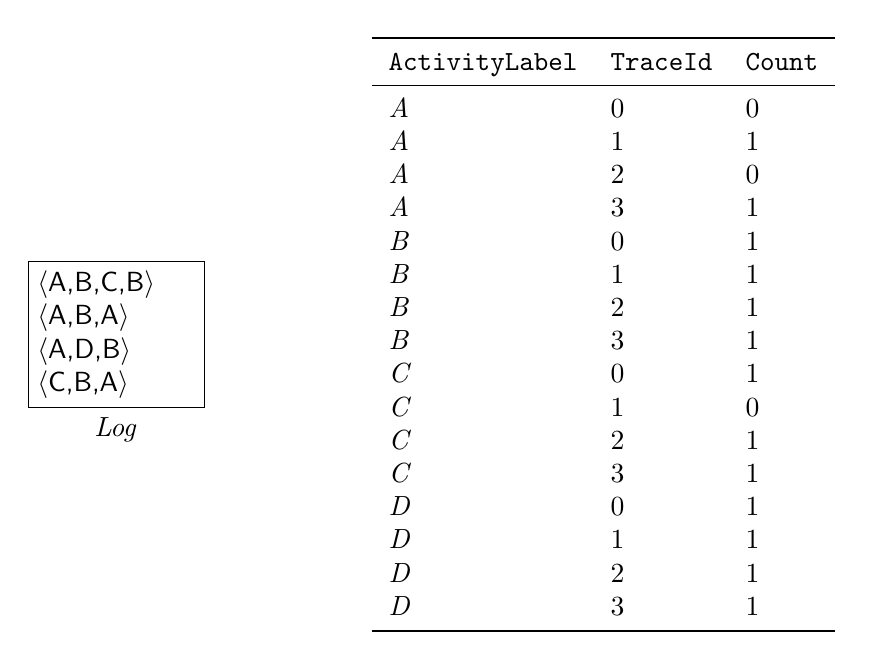
\begin{tikzpicture}[tap/.style args = {#1/#2}{decoration={raise=#1,
                                      text along path,
                                      text align={align=center},
                                      text={#2}
                                      },
              postaction={decorate},
              font=\scriptsize
              },>=latex]

\node[text width=2cm,draw=black,label=below:{\textit{Log}}] (A) {$\braket{\textsf{A,B,C,B}}$ $\braket{\textsf{A,B,A}}$ $\braket{\textsf{A,D,B}}$ $\braket{\textsf{C,B,A}}$} ;

\node[right=2cm of A] (T1) {\begin{tabular}{lll}
\toprule
     \texttt{ActivityLabel} & \texttt{TraceId} & \texttt{Count} \\
\midrule
    \textit{A} & 0 &  0\\
    \textit{A} & 1 &  1\\
    \textit{A} & 2 &  0\\
    \textit{A} & 3 & 1\\
    \textit{B} & 0 & 1\\
    \textit{B} & 1 & 1\\
    \textit{B} & 2 & 1\\
    \textit{B} & 3 &  1\\
    \textit{C} & 0 &  1\\
    \textit{C} & 1 & 0\\
    \textit{C} & 2 & 1\\
    \textit{C} & 3 & 1\\
    \textit{D} & 0 & 1\\
    \textit{D} & 1 &  1\\
    \textit{D} & 2 & 1\\
    \textit{D} & 3 & 1\\
\bottomrule
\end{tabular}};

%\node at (75: 7cm) (csv1) {\includegraphics[width=1cm]{csv.png}};
%\node[below left=.001cm of csv1] (xes1) {\includegraphics[width=1cm]{xes_file_extension.png}};
%\node[draw,fit=(csv1) (xes1),label=below:{``Training'' Log}] (TD) {};
%
%\node at (105: 7cm) (csv2) {\includegraphics[width=1cm]{csv.png}};
%\node[below left=.001cm of csv2] (xes2) {\includegraphics[width=1cm]{xes_file_extension.png}};
%\node[draw,fit=(csv2) (xes2),label=below:{``Testing'' Log}] (TD2) {};
%
%\node[label=below:{Temporal Specification}] at (0: 7cm) (TM) {\includegraphics[width=1.5cm]{report.png}};
%
%\path [->,line width=1.8pt,draw=black, tap={12pt/|\LARGE|Specification Mining}]
%                (TD)    to [bend left] (TM);
%
%
%\node[label=below:{Formal Verification}] at (270: 7cm) (CC) {\includegraphics[width=2cm]{conformance.png}};
%
%\path [->,line width=1.8pt,draw=black]
%                ($(TM.south)-(0,.5cm)$)    to [bend left] (CC);
%\path [->,line width=1.8pt,draw=black]
%                ($(TD2.south)-(0,.5cm)$)    to  (CC);
%
%
%\node[label=below:{Log Repair}] at (180: 7cm) (DR) {\includegraphics[width=2cm]{data_repair.png}};
%\node[label=below:{Specification Repair},right=.5cm of DR] 
% (PR) {\includegraphics[width=2cm]{process_repair.png}};
%
%\path [->,line width=1.8pt,draw=black]
%                (CC)    to [bend left] ($(DR.south)-(0,.5cm)$);
%\path [->,line width=1.8pt,draw=black,tap={12pt/|\LARGE|User Feedback}]
%                (DR)    to [bend left] (TD2);
%
%\path [->,line width=1.8pt,draw=black]
%                (CC)    to [bend left] ($(PR.south)-(0,.5cm)$);
%\draw[->,line width=1.8pt] (PR) edge node [above]{\LARGE{Prediction Adjustment}} (TM);
\end{tikzpicture}
\end{document}